
%!TEX ROOT=ctutest.tex

\chapter{Robot, Simulator}
\label{chapter:robsim}

The first steps in making a robot walk were to select a robot model and a robotics simulator.

In this chapter I will present the selected simulation settings and the reasons that led me to the choice of the simulator and the robot model. 

\section{Simulator Selection}
A robotics simulator is used to create embedded applications for a robot without depending physically on the actual machine, thus saving costs and time. In some cases, these applications can be transferred on the real robot (or rebuilt) without modifications. 

\medskip

I have put together a list of requirements that the simulators would have to fulfill in order to enable me to run the simulation effectively.
\begin{itemize}
\item \textbf{Headless simulation support:} It was clear that it would be necessary to repeat the simulation (episodes) multiple times during the learning process. Headless simulation, meaning running the simulator without GUI, reduces computational costs by not rendering the graphics and also allows remote runs (for example on a server).

\item \textbf{Joints accessible each step of the simulation:} Some simulators do not support this and the joint access is variable, meaning some time steps might be skipped. I opted for simulators with deterministic joint access.

\item \textbf{Open-source license:} Open-source licensing (and available source code) are a must-have when dealing with complex tasks, since they often require at least some code modification of the original release.

\item \textbf{Active community support, documentation:} Lacking thorough documentation and an active community support are often  obstacles for efficient learning and later implementation of the simulation settings. This was a main reason I removed most of the available simulators from the possible candidate list.

\end{itemize}

A good list of viable robotics simulators can be found at \url{https://en.wikipedia.org/wiki/Robotics_simulator}.

From here I chose two possible candidates: \textit{Gazebo} and \textit{V-Rep}.

After many unsuccessful attempts to make Nao model (I allready chose a model at that time) work under Gazebo (there are currently 3 main supported versions of Gazebo and it is not very clear under which the Nao model was supposed to work) I encountered an article \cite{cite:gazebo-vrep} comparing Gazebo and V-Rep in the context of evolution algorithms (a similar setting to reinforcement learning) that recommended V-Rep in terms of user-friendliness and speed.

For these reasons I chose V-Rep as the simulation environment.

\section{Simulation run structure}
V-Rep supports 6 programming languages and I was hoping I could utilize Python machine learning libraries with which I had some experience. Unfortunately the latency between V-Rep's server and Python client turned out to be too large (\textasciitilde 50 ms) for an effective and fast per-step communication.

V-Rep's plugin environment supports per-step communication without delays. Unfortunately, among other flaws (such as slightly confusing v\_repMessage function), one could not send input arguments when running from a console, meaning only one running mode could be run at a time. Because of this, I chose to recompile V-Rep's client from source.

The run structure has changed over time and ended up looking like \ref{fig:langs}.


\begin{figure}
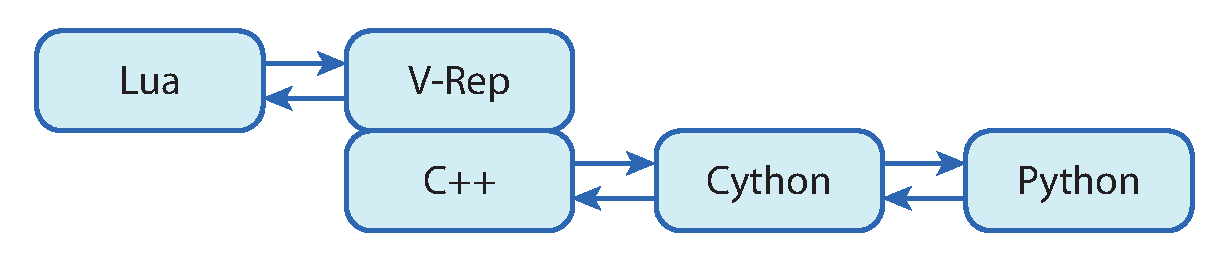
\includegraphics[width=\textwidth]{images/robsim/impl_loop.pdf}
\caption{Main simulation loop}
\label{fig:langs}
\end{figure}

Running V-Rep from console starts a main C++ script that controls access to both the physics engine and the robot control scripts. The C++ script also processes input arguments and switches between different run-types (train, test, etc..).

Each time step, the main script calls some of the control functions that are all written in Cython\footnote{Cython is a programming language that combines C's computational efficiency with Python's high level object-oriented programming. I use it as an interface between the C++ scripts that run the simulator and Python scripts that take care of the machine learning.}.
Some simulation modes also use the V-Rep supported Lua scripts.

\subsection{Simulation details}

The simulator uses several different physics engines (Bullet, ODE, Vortex, Newton), I chose the default Bullet. The control loop is updated every \textit{50}ms, the underlying physics engine loops ten times faster.

One problem across all physics engines is repeatability. In episodic setting the simulation behaves non-deterministically, meaning that repeating the same episode has slightly different outcomes every time. This is caused by the engine's float32 precision and fluctuations in the initial positions.

This problem could be addressed by fully restarting the engine each episodeepisode. However, each restart takes a few seconds which is too long considering that each episode takes most of the time less than a second to complete.

This is why I opted for not restarting fully each episode and instead relied on the learning algorithms to overcome this issue.

\section{Robot}

After a short research of the available humanoid robots I chose the NAO robot for the following reasons:
\begin{itemize}
\item it is one of few humanoid robots commercially available
\item the Faculty of Information Technology, CTU has one model available for students, adding the possibility of future experiments on the physical model
\item its simulation models were available for both V-Rep and Gazebo
\end{itemize}
The robot has 25 degrees of freedom and various sensors including a head camera, an accelerometer, a gyroscope, sonars and more. See figure \ref{fig:nao}.

\begin{figure}[htbp]
\includegraphics[width=.9\textwidth]{images/robsim/nao_joints.jpg}
\caption{The NAO robot joint list\protect\footnotemark}
\label{fig:nao}
\end{figure}
\footnotetext{\label{foot:img-joints}
courtesy of \url{http://doc.aldebaran.com/2-1/family/nao_dcm/actuator_sensor_names.html}}


\subsection{State-Action space}
Because of the nature of the walking task, it is unnecessary to control the head, arms or fingers. Therefore, the upper half of the body has been disabled in the simulator, leaving only the leg and torso joints controllable.

This leaves 12 separate joints (6 for each leg) for control.

While it should be possible to control the robot using joint positions only, it is always beneficial to provide as much information about the state as possible. I have, for this reason, included the joint velocities and 3 accelerometer outputs to the state representation.
\medskip
V-Rep supports joint control in three different ways:
\begin{itemize}
\item \textbf{Position control} V-Rep's most common form of control. Uses an internal PID controller. 
\item \textbf{Velocity control} Mainly a tool used by the position controller, the physics simulator applies maximal torque on the joint, until the desired velocity is reached.
\item \textbf{Torque control} Direct torque control is unfortunately not available, however this can be bypassed by setting the target velocity very high. By setting maximal torque on the joint, the internal physics simulator uses this torque to reach the high velocity, effectively applying torque control.
\end{itemize}

I have used both the position and torque control in the experiments.
